\documentclass{article}
\usepackage[utf8]{inputenc}
\usepackage[free-standing-units=true]{siunitx}
\usepackage{gensymb}
\usepackage{amsmath, amssymb}
\usepackage[T1]{fontenc}
\usepackage{url}
\usepackage{graphicx, caption, subcaption}
\usepackage{minitoc}
\usepackage[font={small,it}]{caption}
\usepackage{float}
\usepackage{multirow}
\usepackage{geometry}
\usepackage{xcolor} % to access the named colour LightGray
\definecolor{LightGray}{gray}{0.9}
\definecolor{grey}{rgb}{0.9,0.9,0.9} % Colour of the box surrounding the title
\definecolor{mygreen}{RGB}{28,172,0} % color values Red, Green, Blue
\definecolor{mylilas}{RGB}{170,55,241}
\usepackage{minted}
\usepackage{booktabs}
\setlength{\parindent}{0px} %makes paragraph indents go away
\usepackage{accents}
\usepackage{listings}
\usepackage{import}
\usepackage{xifthen}
\usepackage{pdfpages}
\usepackage{transparent}
\usepackage[version=4]{mhchem}
% Matrix notation
\newcommand{\matr}[1]{\mathbf{#1}}
\usepackage[font=small,labelfont=bf]{caption}
\usepackage[font=footnotesize]{caption}
\usepackage[british]{babel}
\usepackage{marginnote}

\DeclareSIUnit\angstrom{\text {Å}}
\newcommand\uvec[1]{\underaccent{\vec}{#1}}

\newcommand{\incfig}[1]{%
    \def\svgwidth{\columnwidth}
    \import{./resources/figures/}{#1.pdf_tex}
}

\begin{document}

\pagenumbering{roman}

\begin{titlepage} % Suppresses displaying the page number on the title page and the subsequent page counts as page 1
	
	%------------------------------------------------
	%	Grey title box
	%------------------------------------------------
	
	\colorbox{grey}{
		\parbox[t]{0.93\textwidth}{ % Outer full width box
			\parbox[t]{0.91\textwidth}{ % Inner box for inner right text margin
				\raggedleft % Right align the text
				\fontsize{50pt}{50pt}\selectfont % Title font size, the first argument is the font size and the second is the line spacing, adjust depending on title length
				\vspace{0.7cm} % Space between the start of the title and the top of the grey box
				Monte Carlo Simulation\\
				of Polymers\\
				
				\fontsize{15pt}{30pt}\selectfont
				Simulating polymers as self-avoiding random walks
				\vspace{0.7cm} % Space between the end of the title and the bottom of the grey box
			}
		}
	}
	
	\vfill % Space between the title box and author information
	
	%------------------------------------------------
	%	Author name and information
	%------------------------------------------------
	
	\parbox[t]{0.93\textwidth}{ % Box to inset this section slightly
		\raggedleft % Right align the text
		\large % Increase the font size
		{\Large Francke, A. (4713672)\\ Glorie, M. (4279492)\\ Sangers, J. (4645197)}\\[4pt] % Extra space after name
		Applied Physics - Computational Physics\\
		TU Delft\\
		05-10-2022\\[4pt]
		\hfill\rule{0.4\linewidth}{1pt}% Horizontal line, first argument width, second thickness
	}
	
\end{titlepage}

\begin{abstract}
    \chapter*{Abstract}
This report focusses on utilising scanning transmission electron microscopy in conjunction with a cutting-edge, high dynamic range direct electron detector to acquire precise and localised information on stamped moiré heterostructures. The innovative electron microscope pixelated array detector is employed to capture diffraction data from small areas of heterostructure lattices, generating a four-dimensional dataset. These datasets enable the mapping of strain, electrical, and potential fields with micrometre and nanometre level precision. A novel centre-of-mass analysis approach is developed and integrated into an existing dataset exploration framework for rapid experimentation during electron microscope data acquisition.
\end{abstract}
\newpage
\thispagestyle{empty}
\addcontentsline{toc}{section}{Table of Contents}
\tableofcontents
\clearpage
\newpage
\pagenumbering{arabic}
\section{Introduction}
% \begin{enumerate}

% \item Highlight the significance of working at the nanoscale in terms of technological advancements.

% \item Emphasise that this thesis represents a significant innovation. Mention the unique focus on the integration of 4D-STEM and EMPAD detector.

% \item Clearly state the objectives of the research. Explain the scope, which includes mapping strain, electrostatic potentials, and electric fields in van der waals heterostructures.

% \item Discuss why van der Waals heterostructures is crucial. Emphasise the potential impact on applications. 


% \item Brief outline the methodologies that will be employed, including 4D-STEM

% \item Highlight the contributions of this thesis, such as the development of code for interpreting COM.

% \item Provide an overview of how the thesis is organised, mentioning the subsequent chapters and their roles.
    
% \end{enumerate}


Two-dimensional layered materials have garnered significant attention because they exhibit exciting optical, thermal, and electronic properties that change dramatically as the material is thinned down from bulk to monolayer. The already vast amount of tunability increases even further as one starts to stack these thin two-dimensional building blocks into larger potentially twisted heterostructures. Van der Waals forces that normally hold together the layers in the bulk crystal also form the glue that holds these new heterostructures together. This relative ease in manufacturing and the potential applications in fields ranging from power electronics and solar cells to single-photon emitters and biosensors make studying these materials more than worthwhile~\cite{LI2016322, https://doi.org/10.1002/smll.202107059}.\\
Studying these fascinating materials and the dynamical interplay between the tunable physical properties such as strain, twist angle, and material combination calls for highly sophisticated and specialised characterisation techniques. Therefore, scanning transmission electron microscopy will be used in combination with a state-of-the-art, fast, and high dynamic range direct electron detector to gather highly localised information. The innovative electron microscope pixelated array detector will be used to capture the diffraction information of a small area in the heterostructure crystal lattice by scanning over the sample with a small localised electron probe in a rasterised pattern to form a four-dimensional dataset. From these four-dimensional datasets accurate strain-, electrical-, and potential-fields can be mapped with micrometre and nanometre precision, respectively. To this end a new to us centre-of-mass analysis approach will be developed and implemented in an existing dataset exploration framework used for rapid experimentation of electron microscope parameters at the time of acquisition.\\
In the report, relevant theory on electron microscopy and crystallography will be presented first in Section \ref{sec:theory} after which the fabrication of moiré heterostructures will be explained in Section \ref{sec:methods}. The EMPAD and the data sets it captures and how it will be analysed are explained in Section \ref{sec:empad}. The results stemming from the application of the new analysis techniques are explained in Section \ref{sec:results}, and finally, the conclusions and future possibilities will be discussed in Section \ref{sec:outlook}.


\newpage
\section{Transmission Electron Microscopy and Crystallography of TMDs}

\subsection{The Transmission electron microscope (TEM)}
The Transmission electron microscope (TEM) is a microscope that far exceeds the capabilities of a normal light microscope. Both types of microscope use a series of lenses to magnify the image of a specimen.
A normal light microscope can amplify an image up to about 1500$\times$ and is limited by the diffraction limit of light. Assuming an average wavelength of \SI{550}{\nm} for green light, a high-end microscope is limited to resolving features \SI{100}{\nm} apart.
This limit is insufficient for looking at atomic structures \cite{PhysRevLett.106.193905}.\\
An electron microscope circumvents this limit by using electrons, not light, to probe the specimen. Electrons when accelerated have a smaller wavelength than light thus allowing for images with resolved features as small as \SI{0.05}{\nm}. \cite{kisielowski_freitag_bischoff_van}
The TEM works by releasing electrons from an electron source and accelerating them to an energy typically expressed in kilo-electronvolt; as shown in equation \ref{eq:acc_volts}, the higher the accelerating voltage of the microscope the smaller the de Broglie wavelength of an electron, which results in a higher resolving power. Modern electron microscopes accelerate electrons up to \SI{300}{\kilo \electronvolt}

\begin{equation}
    \lambda_e = h\cdot \left[ 2 \cdot e \cdot m_e \cdot V_a \right]^{-1/2}
    \label{eq:acc_volts}
\end{equation}

\begin{figure}[h]
    \centering
    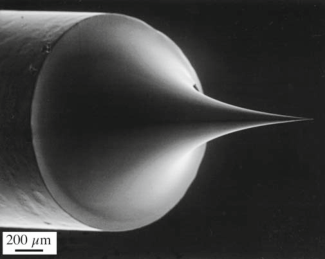
\includegraphics[keepaspectratio, width=0.5\linewidth]{resources/Figures/feg.png} 
    \caption{Pictured is the tip of a field emission gun \cite{Williams2009-ww}. The tapered tip facilitates the creation of a strongly varying potential that eases the expulsion of electrons from the material. These electrons are then accelerated along the optical axis.}
    \label{fig:feg}
\end{figure}

In a TEM the electrons are released from a field emission gun (FEG, pictured in Figure \ref{fig:feg}). 
The FEG is placed in proximity to two anodes, the first anode is positively charged to several kilovolts such that it extracts electrons from the tip of the FEG, the second anode is charged to the wanted acceleration voltage \cite{Williams2009-ww}.
FEGs are about three orders of magnitude brighter than thermionic emission electron sources \cite{field-emission}.
After being emitted the electrons pass through a monochromator that reduces the energy spread of the emitted electrons. An electron then continues along the optical axis into an illuminating system consisting of multiple electromagnetic lenses, which lenses are activated and to what extent depends on the operating mode of the electron microscope.

% \subsubsection{Bright Field}
% A bright field (BF) image of the sample is acquired by using a parallel electron beam. This beam is formed using the lens configuration shown in figure \ref{fig:tem_operating}. This parallel beam is typically several micrometers in size at magnifications up to 20k-100k$\times$.
% In normal operating mode a BF image is captured by a camera looking at a phosphorous screen or by a camera directly, this method of imaging is most analogues to a normal light microscope.
% The electron beam is focused in such a way that it illuminates the sample with a parallel beam, such a beam is also used for creating the clearest diffraction patterns.
% %A bright field image can also be formed in STEM operating mode.
% \begin{figure}[h]
%     \centering
%     \def\svgwidth{.66\linewidth}
%     \import{resources/Figures}{parallel_op_mode.pdf_tex}
%     \caption{Illumination system for parallel beam.}
%     \label{fig:tem_operating}
% \end{figure}
\subsubsection{Dark Field and Z-contrast Imaging}
For dark field and Z-contrast the electron beam is focused to a small area, this creates a higher intensity electron beam with a probe-like point as can be seen in Figure \ref{fig:stem_operating}. Since all the electrons are focused on a small area there is no contrast information that can be used to form an image. To form an image using such a beam the probe point needs to be scanned over the sample leading to the term Scanning Transmission Electron Microscopy.
Dark field images use electrons scattered away from the optical axis to form an image, to achieve this most STEMs have a series of annular dark field detectors.
These ring shaped detectors encircle the central bright field detector and can collect electrons that have been scattered at various angles. Normal dark field detectors collect electrons scattered up to an angle of \SI{50}{\milli \radian}. The outermost detector is the high-angle annular dark field detector (HAADF) which collects electrons scattered beyond \SI{50}{\milli \radian} and can be used to create Z-contrast (atomic number Z) or mass-thickness images.
The HAADF detector is used since the electrons it collects are almost exclusively incoherently elastically scattered which is proportional to the atomic number Z.
The scanning beam then gathers this atomic number information as intensity information for every probe position in the sample.
Layering two monolayers such that the atoms are aligned, and the probe is perpendicularly incident on the sample will sum the intensity of the two atomic weights of the stacked atoms in the image. The stacking pattern can then be determined by looking at a line plot of the atomic mass over atoms.  
\begin{figure}[h]
    \centering
    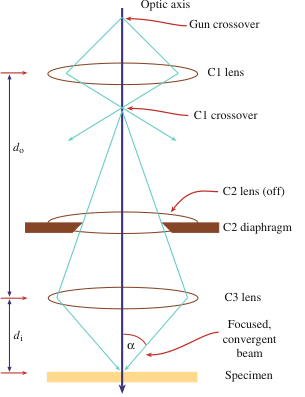
\includegraphics[width=0.5\textwidth, keepaspectratio]{resources/Figures/stem_operating.png}
    \caption{Illumination system for convergent beam.}
    \label{fig:stem_operating}
\end{figure}

% \subsubsection{Energy-dispersive x-ray spectroscopy}
% %Pagina 581 W\&C
% \begin{minipage}[h]{0.6\linewidth}
%         \def\svgwidth{0.66\linewidth}
%         \import{resources/Figures}{Titan_full_column.pdf_tex}
%         \captionof{figure}{Cross-section of an aberration corrected electron microscope}
%         \label{fig:tem_crossection}
% \end{minipage}


\subsection{Crystallography of Transition Metal Dichalcogenides (TMDs)}
\subsubsection{Transition metal dichalcogenides}
Transition metal dichalcogenides or TMDCs are a family of materials consisting of transition metals (group 3 through 12 on the periodic table) and chalcogen atoms (Sulphur, Selenium or Tellurium) in an \ce{MX_2}-configuration, where \ce{M} is the metal atom and \ce{X_2} are the chalcogen atoms \cite{C7TA04268J}.
The properties of TMDCs depend greatly on the amount of stacked layers and with individual layers being as thin as \SI{6.5}{\angstrom} for \ce{MoS_2} these materials are often referred to as layered or two-dimensional materials.
Decreasing the amount of layers from bulk changes electrical properties such as the bandgap which for some TMDCs can go from an indirect to a direct bandgap.
These electrical properties make TMDCs useful in electronics as transistors and in optoelectronics as emitters and detectors \cite{emerg_photolum, LopezSanchez2013, Radisavljevic2011}. 
If present, multiple layers of TMDCs are held together by weak interlayer Van der Waals forces making these materials flexible and transferable using polymer based techniques \cite{reganEmergingExcitonPhysics2022a}.

\subsubsection{Crystal lattice}
An infinitely repeating group of atoms is called an ideal crystal, such a crystal is constructed by attaching the same group of atoms, often called a unit cell, to a lattice.
The lattice can be constructed from $n$ independent lattice vectors. $n=1$ for an atomic chain, $n=2$ for a two-dimensional monolayer, and, $n=3$ for a three-dimensional crystal.
If no smaller repeating group of atoms can be constructed to fill the lattice then this group of atoms is called the primitive unit cell and the $n$-independent lattice vectors are then called the primitive translation vectors $a_{n}$ \cite{Kittel1995-qt}.
Each of the $n$ lattice vectors signifies a direction and length of displacement needed such that the shifted crystal lattice is indistinguishable from the original crystal lattice \ref{eq:lattice_equivalent}.
Lattice vectors are also used to specify the orientation of a crystal plane by denoting where the plane intersects the lattice vectors, this procedure allows for unique indexing of crystallographic planes. The use of these planes will be discussed in \ref{sec:diffraction}.
\begin{equation}
    \vec{r}' = \vec{r} + u_1 \vec{a_1} +u_2 \vec{a_2} + u_3 \vec{a_3}
    \label{eq:lattice_equivalent}
\end{equation}

\subsubsection{Reciprocal lattice and electron diffraction}
\label{sec:diffraction}
In the previous section the crystal lattice was introduced, and it was mentioned that there were unique planes characterized by the points where they intersect the lattice vectors.
In reciprocal space every lattice point is equivalent to one set of these planes.
To best understand a crystal, it is helpful to conceptualize it as having two lattices. The first lattice pertains to the organization of the atoms within the crystal's unit cells. The second lattice is a pattern of points that is specific to each crystal and does not correspond to the atom arrangement. Rather, each point in the lattice is linked to a particular set of planes within the crystal \cite{Williams2009-ww}.
Both lattice constructions are equally valid but are helpful under different circumstances; the reciprocal lattice, for instance, is a useful geometrical construct when talking about diffraction.

The reciprocal lattice, just like the crystal lattice, is constructed by vectors; in the case for the reciprocal lattice these are the reciprocal lattice vectors $\vec{b}_n$.
The reciprocal lattice vectors are constructed from the real-space lattice vectors using equation (\ref{eq:lattice_ortho_norm}) and satisfy relation (\ref{eq:lattice_vec_prop}) with their real-space counterpart.
Using these definitions the reciprocal lattice vectors are unique.
Any reciprocal vector can now be composed uniquely by a linear combination of the reciprocal lattice vectors, such that any vector is scaled and summed. If the scalars are integers they are the miller indices and correspond to a crystallographic plane. \\
Scattering off of these planes shows as a series of high-intensity spots in a diffraction pattern image (Figure \ref{fig:diffraction_pattern}), such an image can be taken in the diffraction mode of a scanning transmission electron microscope (STEM). \\

\begin{minipage}{0.5\textwidth}
    \begin{equation}
        \vec{b}_i = 2 \pi \vec{a}_j \times \vec{a}_k \cdot \left[ \vec{a}_i \cdot ( \vec{a}_j \times \vec{a}_k ) \right]^{-1} 
        \label{eq:lattice_ortho_norm}
    \end{equation}
\end{minipage}%
\begin{minipage}{0.5\textwidth}
    \begin{equation}
        \vec{b}_i \cdot \vec{a}_j = 2\pi \delta_{ij}
        \label{eq:lattice_vec_prop}
    \end{equation}
\end{minipage}\\

In a transmission electron microscope the electrons emanating from the field emission gun are modelled as plane waves. When incident on an atomically thin crystalline sample, the plane waves scatter predictably following the physical criteria that incoming and outgoing electrons beams are plane waves with wave vectors $\vec{k_I}$ and $\vec{k_O}$ for incoming and outgoing waves. The resulting change in wave vector due to the scattering of the sample is then equal to $\vec{K} = \vec{k_I}-\vec{k_O}$. As seen in Figure \ref{fig:scatt_angle}, the outgoing electron beam wavefront is deflected by an angle $\theta$ from the incident electron beam such that both are in phase, this angle is the Bragg angle \cite{Williams2009-ww}; and using that $\vert \vec{k_I} \vert = \vert \vec{k_O} \vert = \vert \vec{K} \vert =\lambda_e^{-1}$, with $\lambda_e$ the electron wavelength, the scattering angle can be expressed as:

\begin{equation}
    \sin{\theta}=\frac{\vert \vec{K}\vert / 2}{\vert \vec{k_I}\vert}
    \label{eq:bragg_angle}
\end{equation}

If both outgoing rays from the same incoming beam wavefront are then in phase, meaning that the extra distance travelled by on of the rays is a multiple of the wavelength, it shows as a bright spot in the image and then the following condition is met for the Bragg angle:

\begin{equation}
    n \lambda_e = 2 d \sin{\theta_B}
    \label{eq:bragg_angle_ser}
\end{equation}

This shows that scattering allows for a finite quantized momentum transfer from the electron to the crystal lattice or vice versa. In a crystalline sample this results in bright spots in the diffraction image, where each bright spot can be indexed and attributed to a family of planes in the crystal that facilitate the momentum transfer for the electrons to reach that spot on the detector or phosphor film.
Just as the real-space lattice has a unit cell so does the reciprocal lattice. In reciprocal space this unit cell is called the Brillouin zone.

\begin{figure}
    \centering
    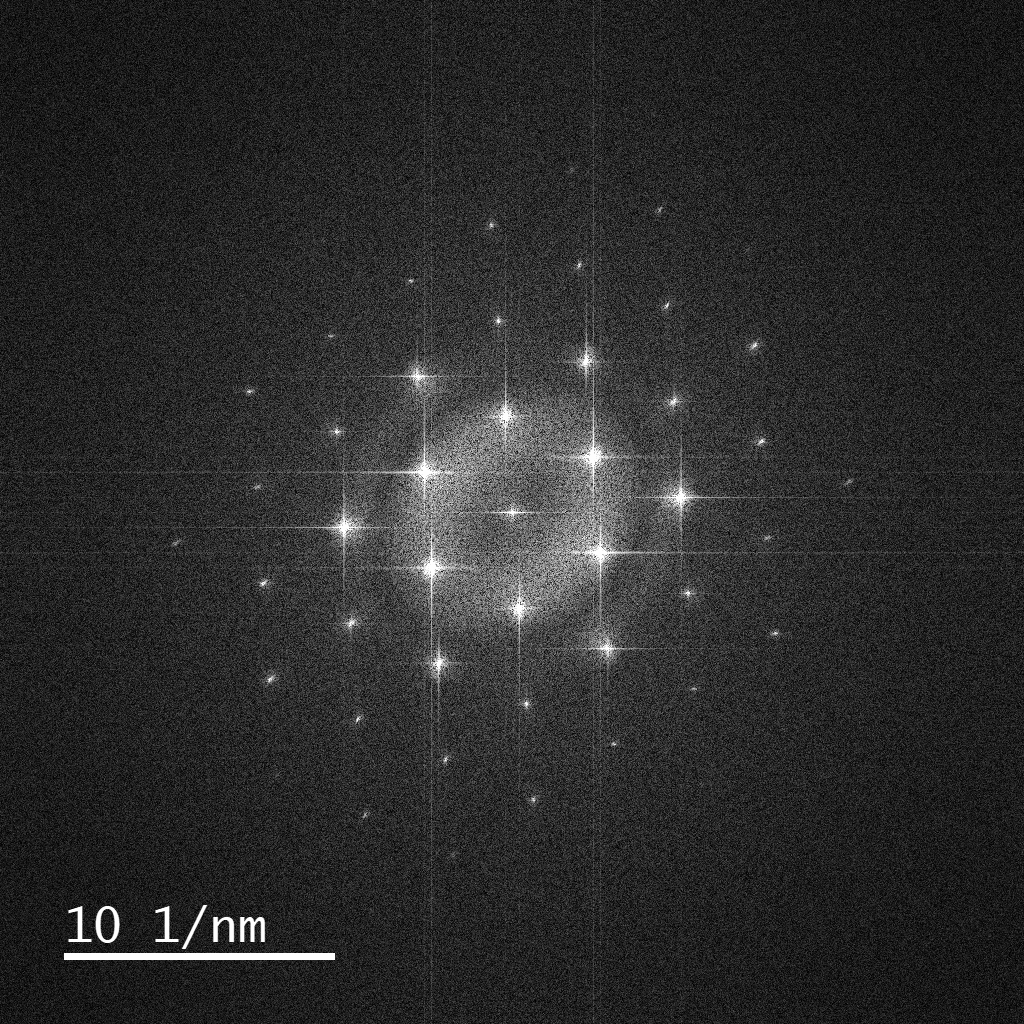
\includegraphics[width=0.3\textwidth, keepaspectratio]{resources/Figures/fft_of_ml.png}
    \caption{Diffraction Pattern}
    \label{fig:diffraction_pattern}
\end{figure}

\begin{figure}
    \centering
    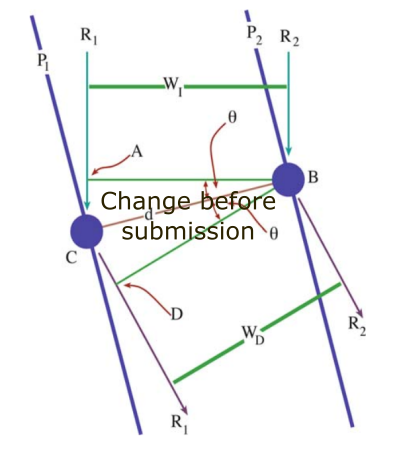
\includegraphics[width=0.3\textwidth, keepaspectratio]{resources/Figures/scattering.png}
    \caption{Scattering diagram}
    \label{fig:scatt_angle}
\end{figure}

\subsubsection{Convergent beam electron diffraction}
In convergent beam electron diffraction the sample is not illuminated by a parallel beam of electrons but instead the electron microscope forms a cone-like shape such that all electrons are focused onto a area only a few atoms wide. The convergence of the electron beam is characterised by the semi-convergence angle $\alpha$ and is usually few to tens of \si{\milli\radian} in size.
Since the local crystal structure is now imaged by a cone-like probe, and not a parallel beam, it is illuminated from multiple different incoming angles; this distribution of incoming angles is then scattered due to the planes in the crystal lattice with the effect of opening the Bragg spots from the previous section to Bragg disks. A typical CBED pattern is displayed in Figure \ref{fig:pacbed}.

\begin{figure}
    \centering
    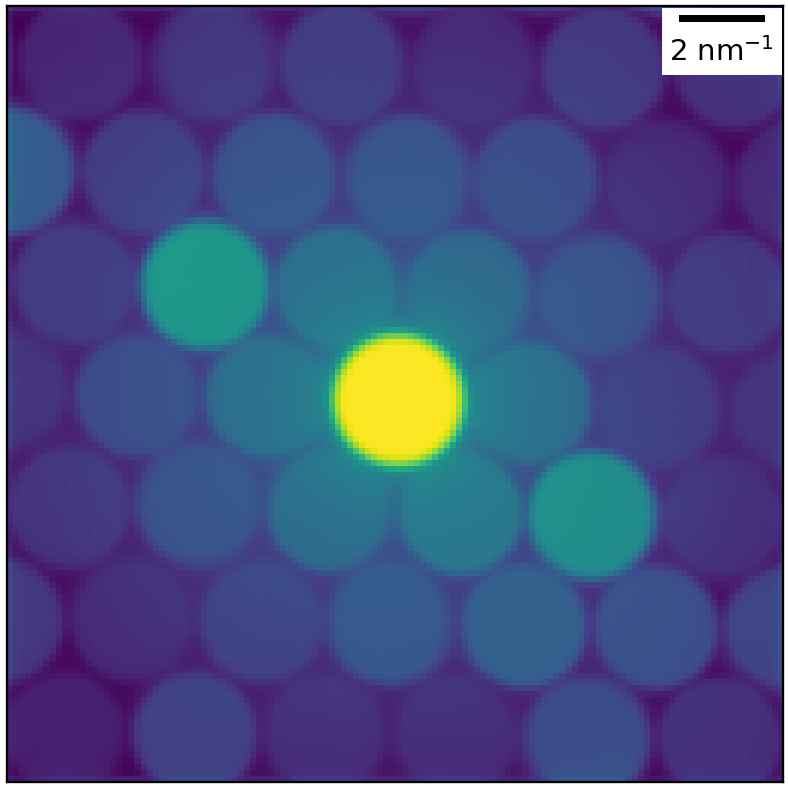
\includegraphics[width=0.5\textwidth, keepaspectratio]{resources/Figures/pacbed_hole.png}
    \caption{A convergent-beam electron diffraction pattern imaged using the EMPAD sensor. Image was calibrated by determining the distance in pixels between Bragg disks and comparing to the FFT of the same crystal imaged using the calibrated CETA camera.}
    \label{fig:pacbed}
\end{figure}

\subsection{Moiré Physics in two-dimensional heterostructures}

\begin{figure}[h]
    \centering
    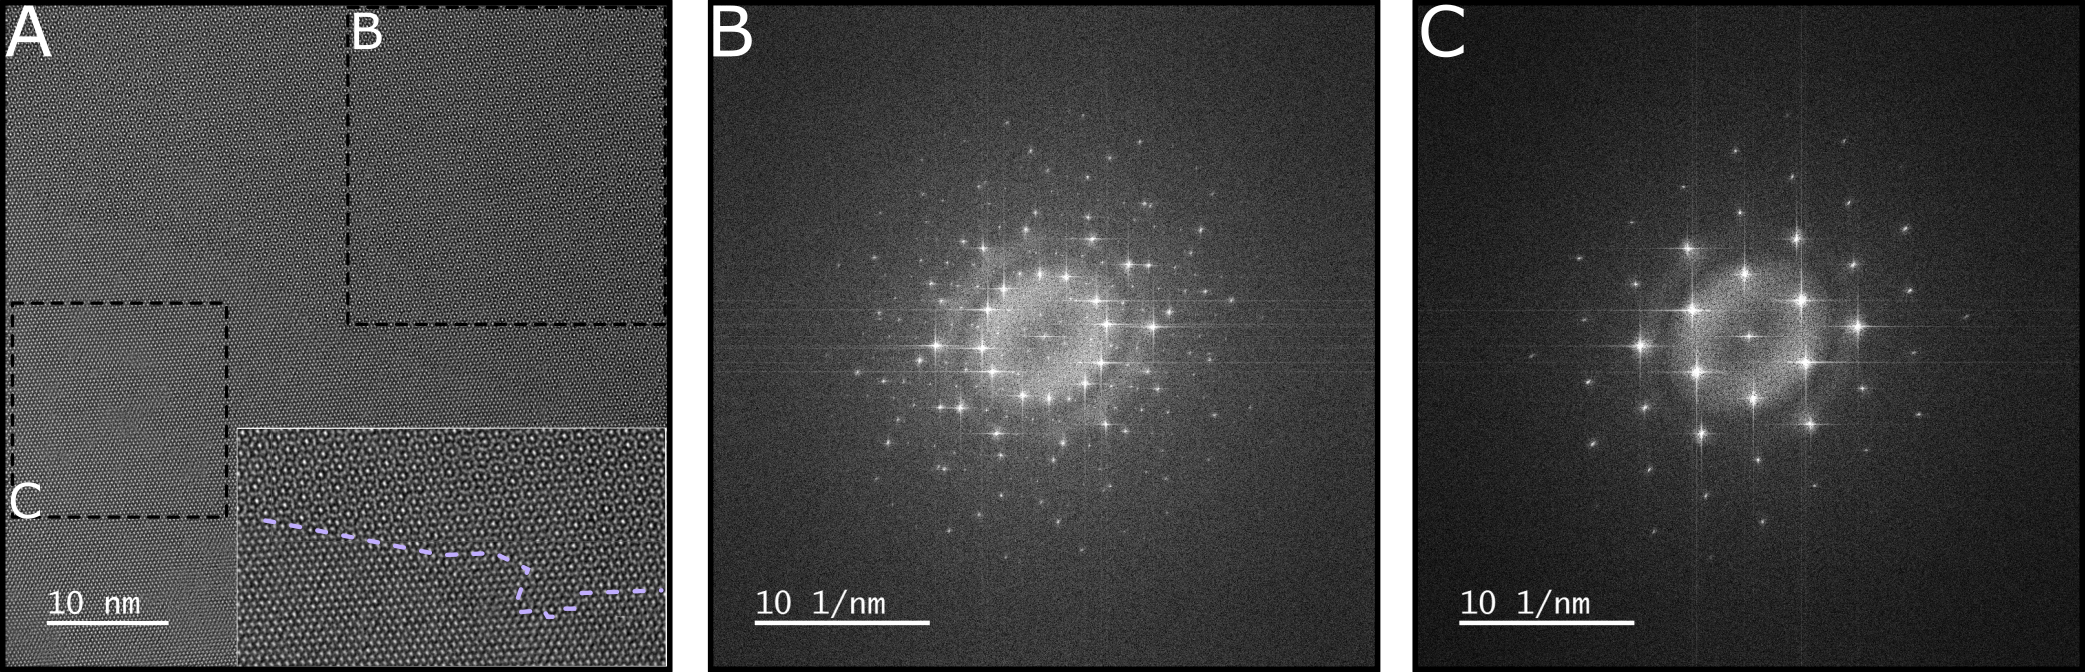
\includegraphics[width=1\linewidth, keepaspectratio]{resources/Figures/moire_transition.png}
    \marginnote{Check detail of Figure \ref{fig:moire_trans}A in print, maybe switch with larger moiré cell} 
    \caption{\textbf{a} High-resolution TEM image of a transition region between singular TMDC material and a twisted heterostructure showing the smallest possible moiré supercell. Dashed regions correspond to subfigures of the same letter, the with white outlined inset is a post-measurement zoomed in image of the transition region with a dashed line guiding the eye towards the flake edge that causes the visual transition. \textbf{b,c} Fast-Fourier transforms of the dashed regions in \textbf{a}. \textbf{b} Shows twelve first-order diffraction peaks indicating that this region consists of two different layers with a roughly \SI{30}{\degree} twist, leading to the smallest possible moiré cell. \textbf{c} Shows six first-order diffraction peaks indicating that its from a single untwisted  crystal. }
    \label{fig:moire_trans}
\end{figure}

Interaction between imaging electrons and crystal lattices lead to the effects described in the previous section, adding a second crystalline structure rotated with respect to the first will affect both lattices as well as create a larger also periodic moiré lattice.
Figure \ref{fig:moire_trans}\textbf{a} shows the transition from single crystal layer to a bilayer region where the constituent layers are rotated from one another, in this bilayer region the effective enlargement of periodic structure is visible as the repeating moiré unit cell is significantly larger than the periodic unit cell of the single layer. The periodicity of the moiré cell is dependent on the rotation between layers and is smallest for \SI{30}{\degree} rotation and increases as the rotation is decreased. The exact periodicity depends on the combination of materials but can be as large as tens of nanometres for transition-metal dichalcogenides with small lattice mismatch \cite{rosenbergerAtomicReconstructionMoire}.

\subsubsection{Diffraction patterns of moiré heterostructures}
The diffraction patterns displayed in Figure \ref{fig:moire_trans}\textbf{b,c} corresponding to the moiré region and the single layer region in Figure \ref{fig:moire_trans}\textbf{a} respectively share some peaks but not all and the extra peaks can not be explained by rotating the diffraction pattern in Figure \ref{fig:moire_trans}\textbf{c} and superimposing in on the pattern in Figure \ref{fig:moire_trans}\textbf{b}.
These extra satellite peaks that emerge between the main Bragg spots and surround the central spot are attributed to the electrons scattering twice, once of off the first layer and then a second time of off the second layer, transferring momentum between the layers while doing so. As these satellite peaks are second order effects they appear dimmer than the main Bragg diffraction spots.
These extra momenta transfer possibilities that open up are displayed schematically in Figure \ref{fig:moire_saed}. In Figure \ref{fig:moire_saed}\textbf{a} the diffraction patterns of two crystal lattice, one red and one blue, are presented; these two lattices each allow six first order momenta transfers by themselves but when brought into proximity the second layer allows scattered electrons to scatter again of its lattice creating the compounded scattering vectors displayed in orange in Figure \ref{fig:moire_saed}\textbf{a,b}. In Figure \ref{fig:moire_saed}\textbf{c} a moiré diffraction pattern is indexed by the cause of the peaks.


\begin{figure}[h]
    \centering
    \def\svgwidth{1\linewidth}
    \import{resources/Figures}{moire_saed.pdf_tex}
    \caption{\textbf{a} Schematic of diffraction patterns of two crystalline samples (red and blue) with a relative twist. The vectors: $\vec{r}_i^n$, $\vec{b}_i^n$, $\vec{c}_i^n$, illustrate the momentum transfers possible due to scattering of a family of planes in the red, blue, or, compound crystal; respectively. In the notation $n$ and $i$ denote the order and the cluster within that order. \textbf{b} Illustration highlighting the new momentum transfer possibilities that open up as two twisted crystalline samples are brought into contact. The newly formed satellite peaks are linear combinations of the intracrystal momentum transfers allowed by the red and/or blue crystal structure and an intercrystal momentum transfers. \textbf{c} Schematic overlaid onto the FFT of a HRTEM image of a moiré cell.}
    \label{fig:moire_saed}
\end{figure}


\section{Methods}
\subsection{Mechanical transfer}
Mechanical transfer relates to the method of moving a sample from one substrate to another whilst minimising the amount of imperfections introduced. This transfer is usually from the growth substrate to a target substrate used for an electrical device or to a TEM grid for characterization in a transmission electron microscope.
\subsection{TEM / EMPAD / EELS? / HRTEM}
\begin{enumerate}
    \item Electron microscope workings and explanation of all detectors
    \item empad detector working / uses
    \item CoM for electric and magnetic fields
    \item charge density mapping
    \item Strain mapping
\end{enumerate}

\subsection{The Transmission electron microscope}
The Transmission electron microscope (TEM) is a microscope that far exceeds the capabilities of a normal light microscope. Both types of microscope use a series of lenses to magnify the image of a specimen.
A normal light microscope can amplify an image up to about 1500$\times$ and is limited by the diffraction limit of light. Assuming an average wavelength of \SI{550}{\nm} for green light, a high-end microscope is limited to resolving features \SI{100}{\nm} apart.
This limit is insufficient for looking at atomic structures \cite{PhysRevLett.106.193905}.\\
An electron microscope circumvents this limit by using electrons, not light, to probe the specimen. Electrons when accelerated have a smaller wavelength than light thus allowing for images with resolved features as small as \SI{0.05}{\nm}. \cite{kisielowski_freitag_bischoff_van}
The TEM works by releasing electrons from an electron source and accelerating them to an energy typically expressed in kilo-electronvolt; as shown in equation \ref{eq:acc_volts}, the higher the accelerating voltage of the microscope the smaller the de Broglie wavelength of an electron, which results in a higher resolving power. Modern electron microscopes accelerate electrons up to \SI{300}{\kilo \electronvolt}

\begin{equation}
    \lambda_e = h\cdot \left[ 2 \cdot e \cdot m_e \cdot V_a \right]^{-1/2}
    \label{eq:acc_volts}
\end{equation}

\begin{figure}[h]
    \centering
    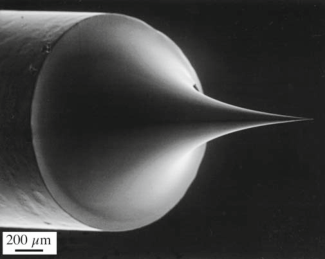
\includegraphics[keepaspectratio, width=0.5\linewidth]{resources/Figures/feg.png} 
    \caption{Pictured is the tip of a field emission gun \cite{Williams2009-ww}. The tapered tip facilitates the creation of a strongly varying potential that eases the expulsion of electrons from the material. These electrons are then accelerated along the optical axis.}
    \label{fig:feg}
\end{figure}

In a TEM the electrons are released from a field emission gun (FEG, pictured in Figure \ref{fig:feg}). 
The FEG is placed in proximity to two anodes, the first anode is positively charged to several kilovolts such that it extracts electrons from the tip of the FEG, the second anode is charged to the wanted acceleration voltage \cite{Williams2009-ww}.
FEGs are about three orders of magnitude brighter than thermionic emission electron sources \cite{field-emission}.
After being emitted the electrons pass through a monochromator that reduces the energy spread of the emitted electrons. An electron then continues along the optical axis into an illuminating system consisting of multiple electromagnetic lenses, which lenses are activated and to what extent depends on the operating mode of the electron microscope.

\subsubsection{Bright Field}
A bright field (BF) image of the sample is acquired by using a parallel electron beam. This beam is formed using the lens configuration shown in figure \ref{fig:tem_operating}. This parallel beam is typically several micrometers in size at magnifications up to 20k-100k$\times$.
In normal operating mode a BF image is captured by a camera looking at a phosphorous screen or by a camera directly, this method of imaging is most analogues to a normal light microscope.
The electron beam is focused in such a way that it illuminates the sample with a parallel beam, such a beam is also used for creating the clearest diffraction patterns.
%A bright field image can also be formed in STEM operating mode.
\begin{figure}[h]
    \centering
    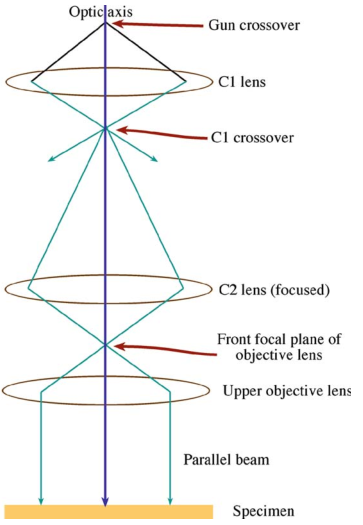
\includegraphics[width=0.3\textwidth, keepaspectratio]{resources/Figures/tem_operating.png}
    \caption{Illumination system for parallel beam.}
    \label{fig:tem_operating}
\end{figure}
\subsubsection{Dark Field, Z-contrast}
For dark field and Z-contrast the electron beam is focused to a small area, this creates a higher intensity electron beam with a probe-like point as can be seen in Figure \ref{fig:stem_operating}. Since all the electrons are focused on a small area there is no contrast information that can be used to form an image. To form an image using such a beam the probe point needs to be scanned over the sample leading to the term Scanning Transmission Electron Microscopy.
Dark field images use electrons scattered away from the optical axis to form an image, to achieve this most STEMs have a series of annular dark field detectors.
These ring shaped detectors encircle the central bright field detector and can collect electrons that have been scattered at various angles. Normal dark field detectors collect electrons scattered up to an angle of \SI{50}{\milli \radian}. The outermost detector is the high-angle annular dark field detector (HAADF) which collects electrons scattered beyond \SI{50}{\milli \radian} and can be used to create Z-contrast (atomic number Z) or mass-thickness images.
The HAADF detector is used since the electrons it collects are almost exclusively incoherently elastically scattered which is proportional to the atomic number Z.
The scanning beam then gathers this atomic number information as intensity information for every probe position in the sample.
Layering two monolayers such that the atoms are aligned, and the probe is perpendicularly incident on the sample will sum the intensity of the two atomic weights of the stacked atoms in the image. The stacking pattern can then be determined by looking at a line plot of the atomic mass over atoms.  
\begin{figure}[h]
    \centering
    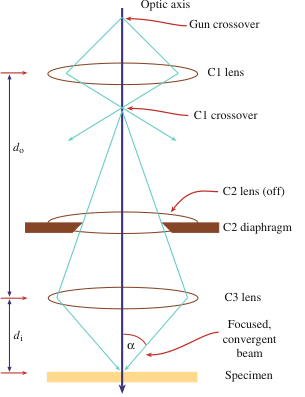
\includegraphics[width=0.5\textwidth, keepaspectratio]{resources/Figures/stem_operating.png}
    \caption{Illumination system for convergent beam.}
    \label{fig:stem_operating}
\end{figure}

\subsubsection{Energy-dispersive x-ray spectroscopy}
Pagina 581 W\&C

\begin{figure}
    \def\svgwidth{.66\linewidth}
    \import{resources/Figures}{Titan_full_column.pdf_tex}
    
\end{figure}

\subsubsection{Electron microscope pixel-array detector}
%In TEM operating mode a parallel electron beam is used to illuminate the sample and form an image on either the phosphorous screen or digital camera, this spreads the beam over a larger area such that the local electron dose is relatively uniform.
In a scanning-TEM (STEM) mode the beam is focused to a small probe-like point at the specimen. Elastic scattering then deflects the electrons from the optical axis onto one of the ring shaped detectors encircling the optical axis, these detectors are called the dark field detectors. These singular annular detectors bunch the elastically scattered electrons together, losing valuable information on the exact scattering angle. The electron microscope pixel-array detector (EMPAD) solves this problem by replacing the annular dark field and singular bright field detectors with a single fast-readout, high dynamic range pixel grid on which every pixels' electron dose is stored separately such that after acquisition of a complete STEM scan the bright- and dark-field detectors can be virtually recreated by integrating the electron dose using annular or circular masks on the data. A greater accuracy in scattering angle is also available since every pixel in the array has its own smaller range of scattering angles whose electrons the pixel collects.



\subsubsection{Electron energy-loss spectroscopy}
In a TEM setup electrons are essentially shot through a sample in which the electrons can either simply pass through or scatter, in the latter scenario there are two possibilities, electrons can scatter elastically or inelastically.
Scattering is a result of the interaction between the sampling electrons from the TEM source and the charged particles in the specimen.\\
When scattering elastically the electrons interact with a nucleus of the specimen whose mass is many times greater than that of the sampling electron, resulting in a small and usually unmeasurable energy transfer.
In a crystalline specimen electrons can only be scattered at certain angles due to the crystal structure creating a diffraction pattern of bright spots. In cases of large scattering angles the electron does transfer a significant amount of energy and can even reverse direction, this energy transfer can permanently displace atoms in the crystal structure causing a defect.\cite{Egerton_2008}\\
When the sampling electron interacts with an electron in the specimen's crystal lattice inelastic occurs due tot the similarity in mass between the two electrons. The energy transfer of this interaction ranges from a few electronvolts up to multiple hundreds of electronvolts.
Inelastic scattering not only results in an energy transfer but also in a momentum transfer as shown in figure \ref{fig:scat}, the $k'$-vector shows a scattered electron that deviates from the not scattered electron vector $k_0$.
The total momentum transfer is the sum of the perpendicular momentum transfer $q_{\perp}$ proportional to the scattering angle $\theta$ and the momentum transfer parallel to the undisturbed path due to an energy transfer from the sampling electron to the sample. This parallel momentum transfer is thus proportional to the energy loss of the electron.
Figure \ref{fig:bands} shows the band structure of the crystalline sample of which the electrons scatter. In this figure two dispersion bands are shown, both bands can be occupied by electrons of certain energies, to excite an electron from the blue band to the red band an electron needs either energy (path $t_1$) or energy and momentum (path $t_2$).
The needed energy and momentum are transferred from an incident sampling electron in the inelastic interaction. By measuring the energy and momentum of a scattered electron it is possible to piece together all the combinations of energy and momenta transfer possible and thus find the band structure of the sample.\\
Another form of inelastic scattering is plasmon excitation.\\
Since the outer-shell electrons of an atom are only weakly bound to the nucleus due to screening effects but are coupled together by electrostatic interaction. These delocalised electrons form an energy band similar to that shown in figure \ref{fig:bands}.
When a fast-moving sampling electron is shot through the sample all nearby outer-shell electrons are displaced. If the sampling electron's velocity exceeds the fermi speed the displacement of outer-shell electrons creates an oscillating ripple creating waves of alternating positive and negative electric charge, this is known as a plasmon wake.\cite{Egerton_2008}

\subsection{Momentum resolved electron energy-loss spectroscopy}
\label{sec:MREELS}
Momentum resolved electron energy-loss spectroscopy hereafter abbreviated as MREELS is a TEM imaging technique in which the imaging plane of the CCD camera is placed in the focal point of the imaging lenses and energy filter.
This allows the camera to take a diffraction mode image in which the diffraction pattern of the scattering electrons is shown. This is illustrated in figure \ref{fig:diff-im}. In this figure the crystalline sample is shown as the box with the slanted lines that represent the Miller planes of the crystal structure.
As shown in the figure all electrons that scatter of the same family of Miller planes get focused on the same region on the imaging sensor, electrons that do not scatter also get focused in one spot at the centre of the diffraction pattern.
A diffraction mode image does not image normal space but instead shows reciprocal space which is also the reason this type of image is useful. In a normal image one would attribute lengths to the axes of an image but in a diffraction mode image the separation of features is given by a momentum difference.
The separation of the light and dark grey arrows on the imaging plane in figure \ref{fig:diff-im} is thus equal to the difference in perpendicular momentum transfer between scattering electrons (light grey) and electrons that do not scatter (dark grey), a 3D representation is presented in the Appendix.
Since the momentum transfer for the electrons that do not scatter is zero the momentum transfer for scattering of a certain family of planes can be determined.

\subsubsection{Energy filtered transmission electron microscope}
\label{sec:eftem}
An energy filtered transmission electron microscope is a microscope with an energy filter placed in the optical column of the TEM. Energy filtering is accomplished by the use of electromagnetic prisms such as those shown in figure \ref{fig:filter}.
These prisms just like ordinary prism disperse the electrons with different wavelengths which are proportional to electron energy. By sliding a slit into the cone of dispersed electrons it is possible to choose a finite range of electron energies to image.
The EFTEM setup can be used in conjunction with the MREELS imaging technique to gather information on both the momentum transfer of the electron (via MREELS) and the energy loss associated (via EFTEM) with that momentum transfer.






\subsection{Data analysis}
\subsubsection{CoM analysis}
\subsubsection{Charge density analysis}
\subsubsection{Strain analysis}





\newpage
\section{Case study of $MoSe_2$/$WSe_2$ moiré heterostructures}

\subsection{Verification of moiré pattern and its parameters}

\begin{figure}
    \centering
    \def\svgwidth{.9\linewidth}
    \import{resources/Figures}{moire_flakes.pdf_tex}
    \caption{(\textbf{a}, \textbf{d}, \textbf{h}) HR-TEM images of three different $MoSe_2$/$WSe_2$-Moiré heterostructures stamped under different angles verified by the FFT of images (\textbf{b}, \textbf{e}, \textbf{i}) taken at $460k\times$ magnification (not shown). The Moiré angle can be determined by measurement of the angle in between the two diffraction peaks in a set, for \textbf{b}, \textbf{e}, \textbf{i} the angle was measured to be $16.6\degree$, $12.2\degree$, and, $8.3\degree$ respectively. (\textbf{c}, \textbf{f}, \textbf{j}) displaying a reconstruction of filtered diffraction patterns, showing a clear Moiré superlattice. The Moiré superlattice cell was measured to be \SI{0.47}{nm}, \SI{1.06}{nm}, and, \SI{1.69}{nm}; for \textbf{c}, \textbf{f}, and, \textbf{j}. (\textbf{a}) The two layers of material show a rough surface that seems to arise during or after transfer to the TEM grid.}
    \label{fig:moire_overview}
\end{figure}

The samples displayed in Figure \ref{fig:moire_overview} have been fabricated using the method outlined in Section \ref{sec:fab_method} but had not been checked under the spectroscope as it had not arrived by then. The flakes were selected for stamping only by using a optical microscope and identifying thin regions. As can be seen in Figure \ref{fig:moire_overview}\textbf{a,d,h} not all flakes are equally thin and are thus not all composed of two layers of monolayer material. The high-resolution TEM images do however show that using the stamping method it is possible to create heterostructures comprised of monolayer material. Figures \ref{fig:moire_overview}\textbf{b,c,f} show the fast Fourier transforms of HRTEM images taken at $460\mathrm{k}\times$ and clearly depict the characteristic double set of Bragg spots that indicate the two crystal layers. Masking the diffraction peaks and taking the inverse Fourier transform then creates a noise-free representation of the moiré lattice (Figure \ref{fig:moire_overview}\textbf{c,f,j}), which shows the expected relation of increasing unit cell for decreasing moiré angles.


\subsection{Analysis of in-plane strain}
\begin{figure}
    \centering
    \def\svgwidth{.74\linewidth}
    \import{resources/Figures}{strain_overview.pdf_tex}
    \caption{Overview of the heterostrain present in both the top and bottom layer of the heterostructure displayed in Figure \ref{fig:moire_overview}\textbf{d} for the left and right column respectively. The red box denotes the reference region for the strain analysis. In any white regions not enough peaks were found to perform strain analysis. \textbf{a,b,e,f}) Show compressive or tensile strain in the top layer for \textbf{a, b} and in the bottom layer for \textbf{e, f}. \textbf{c, g}) illustrate the shear strain in both layers. \textbf{e, h} show the local rotation of the layer with respect to the average rotation in the red box.}
    \label{fig:strain_overview}
\end{figure}

For the analysis of heterostrain the heterostructure displayed in Figure \ref{fig:moire_overview}\textbf{d} was selected as its transfer to the TEM grid went without issue thus leaving no ambiguity in material, whereas for the other two heterostructures depicted in Figure \ref{fig:moire_overview} there were a lot of flakes twirling around in the IPA when dissolving the PVA substrate. The two layers were stamped one on top of another at an angle of \SI{12.2}{\degree} creating a moiré lattice with \SI{1.06}{\nano\meter} periodicity.
The heterostrain analysis was carried out using the exit-wave power cepstrum transform method. Both layers were analysed separately by tracking the corresponding EWPC peaks such that only the strain and rotation within each single layer are considered. In Figure \ref{fig:strain_overview} the results are presented for each layer in their own column. The rows, from top to bottom, denote the compressive/tensile strain in the $x$ and $y$ direction, the shear strain, and, the rotation of the layer; all relative to the reference area denoted by the red square. The rotation in the bottom row is not the same as the moiré angle under which the layers are stamped. The white regions denote the places where the to be tracked peaks were not found, and thus no information could be retrieved.
In Figure \ref{fig:strain_overview}\textbf{a-c, e-d} it is shown that both layers are effected by between \SI{-5}{\percent} and \SI{5}{\percent} strain mostly concentrated near the edges of the supporting carbon mesh over which both layers are draped and for the top layer there also exist strain close to a vertically extending fold in the layer. The relative rotation plot for the top layer shows a stark difference in relative rotation between the left and right side of the fold, meaning that the rotation likely pushed the material in on itself creating the fold. The relative rotation tapers off as the fold also disappears when moving away from the flakes edge as can be seen in Figure \ref{fig:moire_overview}\textbf{b}.\\
\newpage

\section{Case study: An analysis of features in stamped $WSe_2$}
\begin{figure}
    \centering
    \def\svgwidth{.95\linewidth}
    \import{resources/Figures}{e2_overview.pdf_tex}
    \caption{\textbf{a}) High-angle annular dark field photograph, image shows material increasing in layer number from the bottom left to the top right. These layers were slightly rotated during transfer, leading to the formation of the moiré pattern. Across this material another thin strip has settled during transfer causing a further modulation of the moiré period. \textbf{b}) High-resolution TEM image of the region highlighted in \textbf{a} with a moiré unit cell outlined. \textbf{c}) FFT of the high-resolution image showing a \SI{2.3}{\degree} rotation between the strip and larger layers.}
    \label{fig:dub_moire}
\end{figure}

This sample of stamped $WSe_2$ was created using the described mechanical transfer technique and was originally considered unsuccessful as the stamped flakes got jostled up during transfer negating any effort put into alignment of the flakes. Upon inspection in STEM mode the large features highlighted with the green outline in Figure \ref{fig:dub_moire}\textbf{a} appeared and are the effect of three different layers of material slightly out of alignment with one another. The resulting moiré unit cell is highlighted with the dashed outline in Figure \ref{fig:dub_moire}\textbf{b} and is measured to be caused a \SI{2.3}{\degree} rotation between the thin strip's crystal lattice (highlighted in green) and the moiré pattern present in the underlying layers (highlighted in blue).
In the following sections three regions from the previously introduced sample will be looked at: a hole in otherwise uniform material to verify the centre-of-mass analysis tools, a large periodicity moiré lattice to see what can be expected, and finally, the double misaligned region.

\subsection{Hole}

\begin{figure}
    \centering
    \def\svgwidth{.95\linewidth}
    \import{resources/Figures}{hole_displacement.pdf_tex}
    \caption{Result of performing CBED shift analysis on a large hole in otherwise uniform material. \textbf{a,b,c,d}) Highlight the shift in the y-direction, the shift in the x-direction, the magnitude of the shift, and, the angle of the displacement respectively. All values are given are (sub)pixel shifts across the sensor. The axes correspond with those given in the vHAADF image \textbf{e}.}
    \label{fig:hole_dis}
\end{figure}

As highlighted in the previous theory section on centre-of-mass (COM) analysis there are two different scenarios in which one needs to consider different effects on the diffracted electron beam and one thus needs to consider different analysis approaches to the COM analysis. One such scenario is one in which the electron probe's cross-sectional area is much smaller than the feature being imaged, which is the case for the hole in the otherwise uniform moiré bilayer depicted in Figure \ref{fig:hole_dis}\textbf{e}. As reported in other works, changes in sample geometry such  as edges and slopes can deflect the electron bundle. This deflection is towards the thicker region in the sample \cite{ophusFourDimensionalScanningTransmission2019a,dekkers1974differential}. By tracking the edge of the bright field disk and its deviation with respect to its mean position it is possible to recover the deflection of the diffraction pattern in both the $x$- and $y$-direction. This deflection in the $x$- and $y$-deflection is plotted in Figure \ref{fig:hole_dis}\textbf{a,b} and the combined deflection magnitude and deflection angle in Figure \ref{fig:hole_dis}\textbf{c,d} respectively. The effects are as expected with the electron beam displacements being towards the material. There also appear to be a few probe points in the centre of the hole were barely any displacement is measured indicating that the beam's cross-sectional area is indeed smaller than that of the hole. Using the information on the displacement of the diffraction pattern it is also possible to compute the momentum transfer imparted on the electron beam using similar methods as described in \cite{mullerAtomicElectricFields2014}. The net momentum transfer and its direction is plotted in Figure \ref{fig:hole_mom} as well as a virtual-HAADF image for reference. The plot shows higher momenta transfer for probe positions nearer to the hole's edge and tapers of as the probe moves further over the sample or more towards the centre of the hole.

\begin{figure}
    \centering
    \def\svgwidth{.7\linewidth}
    \import{resources/Figures}{hole_momentum_transfered.pdf_tex}
    \caption{Left panel show a virtual-HAADF image taken by masking the dataset. Right panel shows the momentum transfer imparted on the electron beam by the sample, the electron beam gets deflected towards the thicker material.}
    \label{fig:hole_mom}
\end{figure}

\subsection{Small Moiré}

\begin{figure}
    \centering
    \def\svgwidth{.95\linewidth}
    \import{resources/Figures}{moire_displacement.pdf_tex}
    \caption{Result of performing CBED shift analysis on the region of a moiré lattice highlighted in blue in Figure \ref{fig:dub_moire}. \textbf{a,b,c,d}) Highlight the shift in the y-direction, the shift in the x-direction, the magnitude of the shift, and, the angle of the displacement respectively. All values are given are (sub)pixel shifts across the sensor. The axes correspond with those given in the vHAADF image \textbf{e}.}
    \label{fig:m_dis}
\end{figure}


\begin{figure}
    \centering
    \def\svgwidth{.5\linewidth}
    \import{resources/Figures}{moire_efield_charge.pdf_tex}
    \caption{}
    \label{fig:m_mom}
\end{figure}

\subsection{Large Moiré}

\begin{figure}
    \centering
    \def\svgwidth{.95\linewidth}
    \import{resources/Figures}{trip_moire_displacement.pdf_tex}
    \caption{CBED shift analysis performed on the double moiré region highlighted in Figure \ref{fig:dub_moire}. \textbf{a,b,c,d}) Highlight the shift in the y-direction, the shift in the x-direction, the magnitude of the shift, and, the angle of the displacement respectively. All values are given are (sub)pixel shifts across the sensor. The axes correspond with those given in the vHAADF image \textbf{e}.}
    \label{fig:trip_m_dis}
\end{figure}

\begin{figure}
    \centering
    \def\svgwidth{.7\linewidth}
    \import{resources/Figures}{trip_moire_momentum.pdf_tex}
    \caption{Image shows the momentum transfer imparted on the electron beam by features in the sample. The moiré unit cell is highlighted and the same as in Figure \ref{fig:dub_moire}\textbf{b}.}
    \label{fig:trip_m_mom}
\end{figure}


\newpage
\section{Conclusions and Outlook}
\label{sec:outlook}
The stamping and mechanical transfer steps outlined in this report have been demonstrated to have produced at least a single large scale \SI{1}{\micro\meter} heterobilayer structure whose moiré angle was not yet controlled. This has shown that the method, although tedious and once improved upon, has the potential for rapid prototyping of heterostructures with varying material makeup, material thicknesses, moiré twist angle, and possibly in the future even strain. The feasibility of the spectroscopy set-up to identify material and its thickness has been proven to be sufficient for the characterisation and selection of TMD flakes. The wet transfer steps first attempted in this group for the transfer of heterostructures from silicon to holey carbon grids has been improved with time and experience, such that going forward a higher success rate can be achieved.\\
The EMPAD has been successfully employed to characterise the heterostrain in both stacked layers of a heterostructure with a moiré angle of \SI{12.2}{\degree} for large field-of-view. The strain analysis technique utilising the exit-wave power cepstrum transform has proved powerful in dealing with unfavourable features commonly found in stamped and stacked heterostructures like substrates and sample tilt. The centre-of-mass analysis on the EMPAD data has opened up a new possibility for characterising our stamped heterostructures' electric and magnetic potentials at the moiré length scales and was able to disentangle the signal coming from differently sized features. Further thought and experiments will be needed to gain the necessary expertise and intuition required for effectively selecting the feature size whose data is being captured at the time of acquisition.

Overall, the processes implemented in this report lay the groundwork for the prototyping of new heterostructures and find the link between physical characteristics, like strain and twist, and the electronic and magnetic properties of these materials. With the future help of machine learning to better analyse the vast quantities of data gathered by the EMPAD, it will be possible to design and manufacture more sophisticated quantum systems.

%\input{chapters/examples}

\newpage
\addcontentsline{toc}{section}{References}
\bibliographystyle{ieeetr}
\bibliography{resources/literature.bib}

\end{document}
